%! TeX program = xelatex
\documentclass{article}
\usepackage{amsmath}
\usepackage{amssymb}
\usepackage{fontspec}
\usepackage{graphicx}
\usepackage{tikz}
\usepackage[normalem]{ulem}
\usepackage[margin=0.75in]{geometry}

\graphicspath{{../../}, {../../../}}

\setmainfont{Noto Serif CJK KR}
\title{3-4. 명제 step C 풀이}
\author{
    \includegraphics[scale=0.25]{logo}
}
\date{}

\begin{document}
\maketitle

\paragraph{1번}
$f(x)g(x) > 0$이려면 $f(x) > 0, g(x) > 0$이거나, $f(x) < 0, g(x) < 0$이어야 하므로, 구하는 진리집합은 \underline{$(A \cap B) \cup (C \cap D)$}

\paragraph{2번}
$A(q, p) \cup A(~p, q)$는 $q \to p$나 $~p \to q$의 반례의 집합이다. \newline

$q \not\to p$를 보이는 집합은 $Q - P$이고, $~p \not\to q$를 보이는 집합은 $P^C - Q$이므로 구하는 집합은

\[
    (Q - P) \cup (P^C - Q) = \{3, 6\} \cup \{7, 8\} = \underline{\{3, 6, 7, 8\}}
\]

\paragraph{3번}
조건에 의해 $p(n)$에서 $n$이 소인수로 2와 3만 가질 때, $p(n)$은 참이다. 주어진 보기 중 $180 = 2^2 \times 3^2 \times 5$이므로 정답은 \underline{4}번이다.

\paragraph{4번}
수직선을 그려보자. $p$가 $q$이기 위한 충분조건, 즉 $p \to q$이려면 수직선을 그릴 때 다음과 같아야 한다.

\begin{center}
    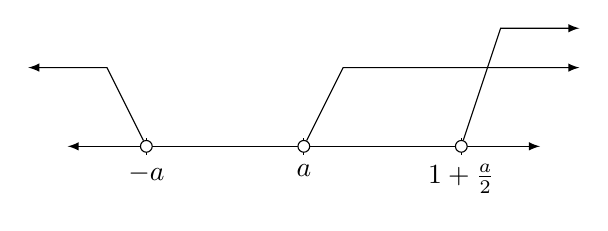
\begin{tikzpicture}
        \draw[latex-latex] (0, 0) -- (6, 0);
        \draw[shift={(1, 0)}, color=black] (0pt, 3pt) -- (0pt, -3pt) node[below] {$-a$};
        \draw[shift={(3, 0)}, color=black] (0pt, 3pt) -- (0pt, -3pt) node[below] {$a$};
        \draw[shift={(5, 0)}, color=black] (0pt, 3pt) -- (0pt, -3pt) node[below] {$1 + \frac{a}{2}$};
        \node[circle,draw,fill=white,inner sep=1.5pt](a)at(1,0){};
        \node[circle,draw,fill=white,inner sep=1.5pt](b)at(3,0){};
        \node[circle,draw,fill=white,inner sep=1.5pt](c)at(5,0){};
        \draw[-latex,black] (a)--++(-0.5,1)--++(-1,0);
        \draw[-latex,black] (b)--++(0.5,1)--++(3,0);
        \draw[-latex,black] (c)--++(0.5,1.5)--++(1,0);
    \end{tikzpicture}
\end{center}

이런 관계가 나오려면 $a > 0$일 때 $1 + \frac{a}{2} \ge a$여야 하고, $a < 0$일 때 $1 + \frac{a}{2} \ge -a$여야 한다. 부등식을 풀면 $a$의 범위는 \underline{$0 < a \le 2$ 또는 $-\frac{2}{3} \le a < 0$}여야 한다.

\paragraph{5번}
모든 실수 $x$에 대해 $5tx^2 - 2tx + 1 \ge 0$이므로 $f(x) = 5tx^2 - 2tx + 1$일 때, 이차방정식 $f(x) = 0$은 중근을 가지거나, 두 허근을 가져야 한다. 이 이차방정식의 판별식을 $D$라 할 때,

\[
    D = (-2t)^2 - 4 \cdot 5t \cdot 1 = 4t^2 - 20t \ge 0
\]

이 부등식을 풀면 $0 \le t \le 5$이고, 앞서 말했듯 $f(x)$는 이차식이므로 $t \not = 0$, 따라서 $t$의 범위는 $0 < t \le 5$이다. \sout{이거 잘못해서 틀림 $\pi\pi$} \newline

또한, $x^2 + (t - 4)x + 1 = 0$의 서로 다른 두 근이 모두 양수가 되어야 하므로 판별식을 $D$라고 할 때

\[
    D = (t - 4)^2 - 4 = t^2 - 8t + 12 > 0
\]

이 부등식을 풀면 $t < 2$ 또는 $t > 6$이고, 따라서 조건을 만족하는 정수 $t$는 1뿐이므로 정답은 \underline{1}.

\end{document}
